\documentclass[]{article}
\usepackage{amsmath}
\usepackage{amsfonts} 
\usepackage[english]{babel}
\usepackage{amsthm}
\usepackage{mathtools}
\usepackage{hyperref}
% \usepackage{minted}
% Basic Type Settings ----------------------------------------------------------
\usepackage[margin=1in,footskip=0.25in]{geometry}
\linespread{1}  % double spaced or single spaced
\usepackage[fontsize=12pt]{fontsize}

\theoremstyle{definition}
\newtheorem{theorem}{Theorem}       % Theorem counter global 
\newtheorem{prop}{Proposition}[section]  % proposition counter is section
\newtheorem{lemma}{Lemma}[subsection]  % lemma counter is subsection
\newtheorem{definition}{Definition}
\newtheorem{remark}{Remark}[subsection]


\hypersetup{
    colorlinks=true,
    linkcolor=blue,
    filecolor=magenta,
    urlcolor=cyan,
}
\usepackage[final]{graphicx}
\usepackage{listings}
\usepackage{courier}
\lstset{basicstyle=\footnotesize\ttfamily,breaklines=true}
\newcommand{\indep}{\perp \!\!\! \perp}
\usepackage{wrapfig}
\graphicspath{{.}}
\usepackage{fancyvrb}

%%
%% Julia definition (c) 2014 Jubobs
%%
\usepackage[T1]{fontenc}
\usepackage{beramono}
\usepackage[usenames,dvipsnames]{xcolor}
\lstdefinelanguage{Julia}%
  {morekeywords={abstract,break,case,catch,const,continue,do,else,elseif,%
      end,export,false,for,function,immutable,import,importall,if,in,%
      macro,module,otherwise,quote,return,switch,true,try,type,typealias,%
      using,while},%
   sensitive=true,%
   alsoother={$},%
   morecomment=[l]\#,%
   morecomment=[n]{\#=}{=\#},%
   morestring=[s]{"}{"},%
   morestring=[m]{'}{'},%
}[keywords,comments,strings]%
\lstset{%
    language         = Julia,
    basicstyle       = \ttfamily,
    keywordstyle     = \bfseries\color{blue},
    stringstyle      = \color{magenta},
    commentstyle     = \color{ForestGreen},
    showstringspaces = false,
}



\begin{document}
\section*{Notations}
\begin{itemize}
    \item [1.] $P_G(u, v)$ a path, which is a list of vertices, or edges, or both, that starts with the vertex $u$ and ends with vertex $v$ in the graph G. 
    \item [2. ] $\text{cc}(v)$ Denotes the connected component, is the set of all rechable vertices from a vertex $V$ in $G$. $G$ can be directed or undirected. It can also be applied to a set of vertices: $S$, which is just $\text{cc}(S):= \bigcup_{v\in S}\text{cc}(v)$
\end{itemize}
\numberwithin{equation}{subsection}
\section{Problem 3.19}
    \begin{prop}[Minimal Bipartite Vertex Cover from Maximum Matching]\label{prop:konig}
        Given a maximum matching on bipartite graph: $G=(U\dot\cup V, E)$ let $M^+$ be a matching of maximum size. 
        \par
        Suppose that solution of a maximum is given after the execution of the matching algorithm and $e\in M$ goes from $U$ to $V$, and $\not\in M$ goes from $V$ to $U$. To get the minimum vertex cover:
        \par
        We choose every reachable vertices from $L$ that is in $V$ (Name that set $S$). Which are going to be covered by $M$. For the remaining vertices that is covered by $M$ and not sharing the same edge in the matching with vertices in $S$, choose then as well, and they will form a vertex cover $F$ with $|F| = |M|$. 
    \end{prop}
    Define the sets and directed edges in the following way: 
    \begin{align}
        & M::\text{The maximum Matching!}
        \\
        & L := \left\lbrace
            v\in U: v\not \in \bigcup_{e\in M} e
        \right\rbrace
        \\
        & S := \text{cc}(L)\cap V
        \\
        & e\in M, e=(v_1, v_2) \implies v_1\in V, v_2\in U
        \\
        & e\not\in M, e=(v_1, v_2) \implies v_1\in U, v_2\in V
    \end{align}
    \begin{enumerate}
        \item [(1.0.2)]: $L$ is the set of vertices in $U$ that are not covered by the matching. 
        \item [(1.0.3)]: $S$ is the set of reachable vertices from all vertices in $L$.  
        \item [(1.0.4)]: An edge in matching goes from $V$ to $U$. 
        \item [(1.0.5)]: an edge not in matching goes from $U$ to $V$. 
    \end{enumerate}
    % \begin{lemma}[Lemma 1]\label{lemma:konig_1}
    %     $U\setminus L$ are all covered by matching $M$. 
    % \end{lemma}
    % \begin{proof}
    %     This is direct by the definition for $L$ (1.0.1) that it's the set of vertices covered by $M$ and it's in $U$. $U\setminus L$ are the rest of these vertices which must be covered by $M$
    % \end{proof}
    \begin{lemma}[Lemma 2]\label{lemma:konig_2}
        It's impossible to have a path going from $L$ to $S$ to $U\setminus L$ to $V\setminus S$. 
    \end{lemma}
    \begin{proof}
        This is true because $S$ by definition is set of all vertices reachable from $L$ in $V$.  And if we reached some vertices in $V\setminus S$, then it's not in $S$, which violate the definition of $S$. 
    \end{proof}
    \begin{lemma}[Lemma 3]\label{lemma:konig_3}
        All vertices in $S$ are covered by $M$. 
    \end{lemma}
    \begin{proof}
        If not, there exists a path going from $u\in L$ to $v\in S$ such that $v$ not covered by $M$, since $u$ not covered by $M$ by definition of $L$; an augmented path is found, therefore $M$ is not maximum. 
    \end{proof}
    \begin{lemma}[Lemma 4]\label{lemma:konig_4}
        No edges, in any directions exists between the set $V\setminus S$, $L$.
    \end{lemma}
    \begin{proof}
        
        For contradiction, suppose there is such an edge and denote that edge as $e^+$. Then the contradiction is: 
        \begin{align}
            e^+ \not \in M \wedge e^+\in M
        \end{align}
        Because $V\setminus S$ is the set of vertices in $V$ that can't be reached by $L$, therefore there are no direct edges going from $L\subseteq U$ to $(V\setminus S)\subseteq V$, therefore, $e^+\not\in M$; which also means $e^+$ will go from $(V\setminus S)\subseteq V$ to $L\subseteq U$, therefore $e^+\in M$. Which is impossible because by definition $L$ is not covered by $M$.
    \end{proof} 
    \begin{proof}[Proposition \ref*{prop:konig}]
        Let $\overline{F}:= U\setminus L$. The claim is the I can keep the $|\overline{F}|$ fixed and exchange vertices to make this into a vertex cover. 
        \par
        If $L= \emptyset$, then $\overline{F}$ is a vertex cover because $\overline{F} = U$. Using the fact that $G$ is bipartite, $\overline F$ covers all edges. And that means $M$ covers all $U$ because $L=\emptyset$; implying $|\overline{F}| = |M|$
        \par
        If $L\neq \emptyset$, then for all $e\in E, e = \{u, v\}$ (direction doesn't matter). Then there are 3 cases: 
        \begin{enumerate}
            \item [(1.)] $e$ goes from $u\in L$ to $v\in S$, let $e=(u, v)$. $e\not \in M$ because $u\in L$ by def of $L$, $u$ not covered by $M$. However, $v$ is covered by $M$ because $v\in S$ and we use \hyperref[lemma:konig_3]{lemma \ref*{lemma:konig_3}}. Therefore $\exists! u'\in U\setminus L: \{u', v\}\in M$. 
            \par
            I can then construct $\overline{F}:= (F\setminus\{u'\})\cup \{v\}$ to be a minimum vertex cover, without losing edges. $u'$ can be removed from $\overline{F}$ by \hyperref[lemma:konig_2]{lemma \ref*{lemma:konig_2}}. To convince you further, assuing it's not the case, suppose that removing $u'$ expose an edge $e'=(u', v')$ that I am unbale to cover. Observe that $v'$ must be in $V\setminus S$ because $S$ are already all covered by $M$. Then the path is possible: 
            \begin{align}
                & u\rightarrow v\rightarrow u' \rightarrow v'
                \\
                & u\in L
                \\
                & v\in S
                \\
                & u' \in U\setminus L
                \\
                & v'\in V\setminus S
            \end{align}
            Which contradicts \hyperref[lemma:konig_2]{lemma \ref*{lemma:konig_2}}. Therefore $(F\setminus\{u'\})\cup \{v\}$ now covers the additional edge: $e$. 
            \item [(2.)] $e=\{u, v\}$, direction doesn't matter, it goes between $S$ and $U\setminus L$. Then $\overline{F}$ covers the edge: $e$ because $v\in U\setminus L$, and $\overline F = U\setminus L$ at the start, and in case (1.), we move vertices to $S$, therefore, such an edge is always gonna be covered by $\overline F$. 
            \item [(3.)] $e$ goes between $U\setminus L$ and $V\setminus S$. This is covered by $\overline F$ because $U\setminus L$ originally covers all vertices in $V\setminus S$, and in case (1.) above, when we remove $u'$, we never expose any edges going between $U\setminus L$ and $V\setminus S$. 
            \item [(4.)] $e$ goes between the set $L$ and $V\setminus S$. This is impossible by \hyperref[lemma:konig_4]{\ref*{lemma:konig_4}}. 
        \end{enumerate}
        For all cases, I can re-arrange $\overline F$ such that its cardinality remains unchanged and all the edges are covered. I started with $|\overline F| = |M|$, therefore, we have a vertex cover $|\overline{F}| = |M|$ in the end. 
        \par
        HEEEEEEY! Here is picture to get my point across \hyperref[fig:1]{fig: \ref*{fig:1}}:
        \begin{figure}[h]\label{fig:1}
            \centering
            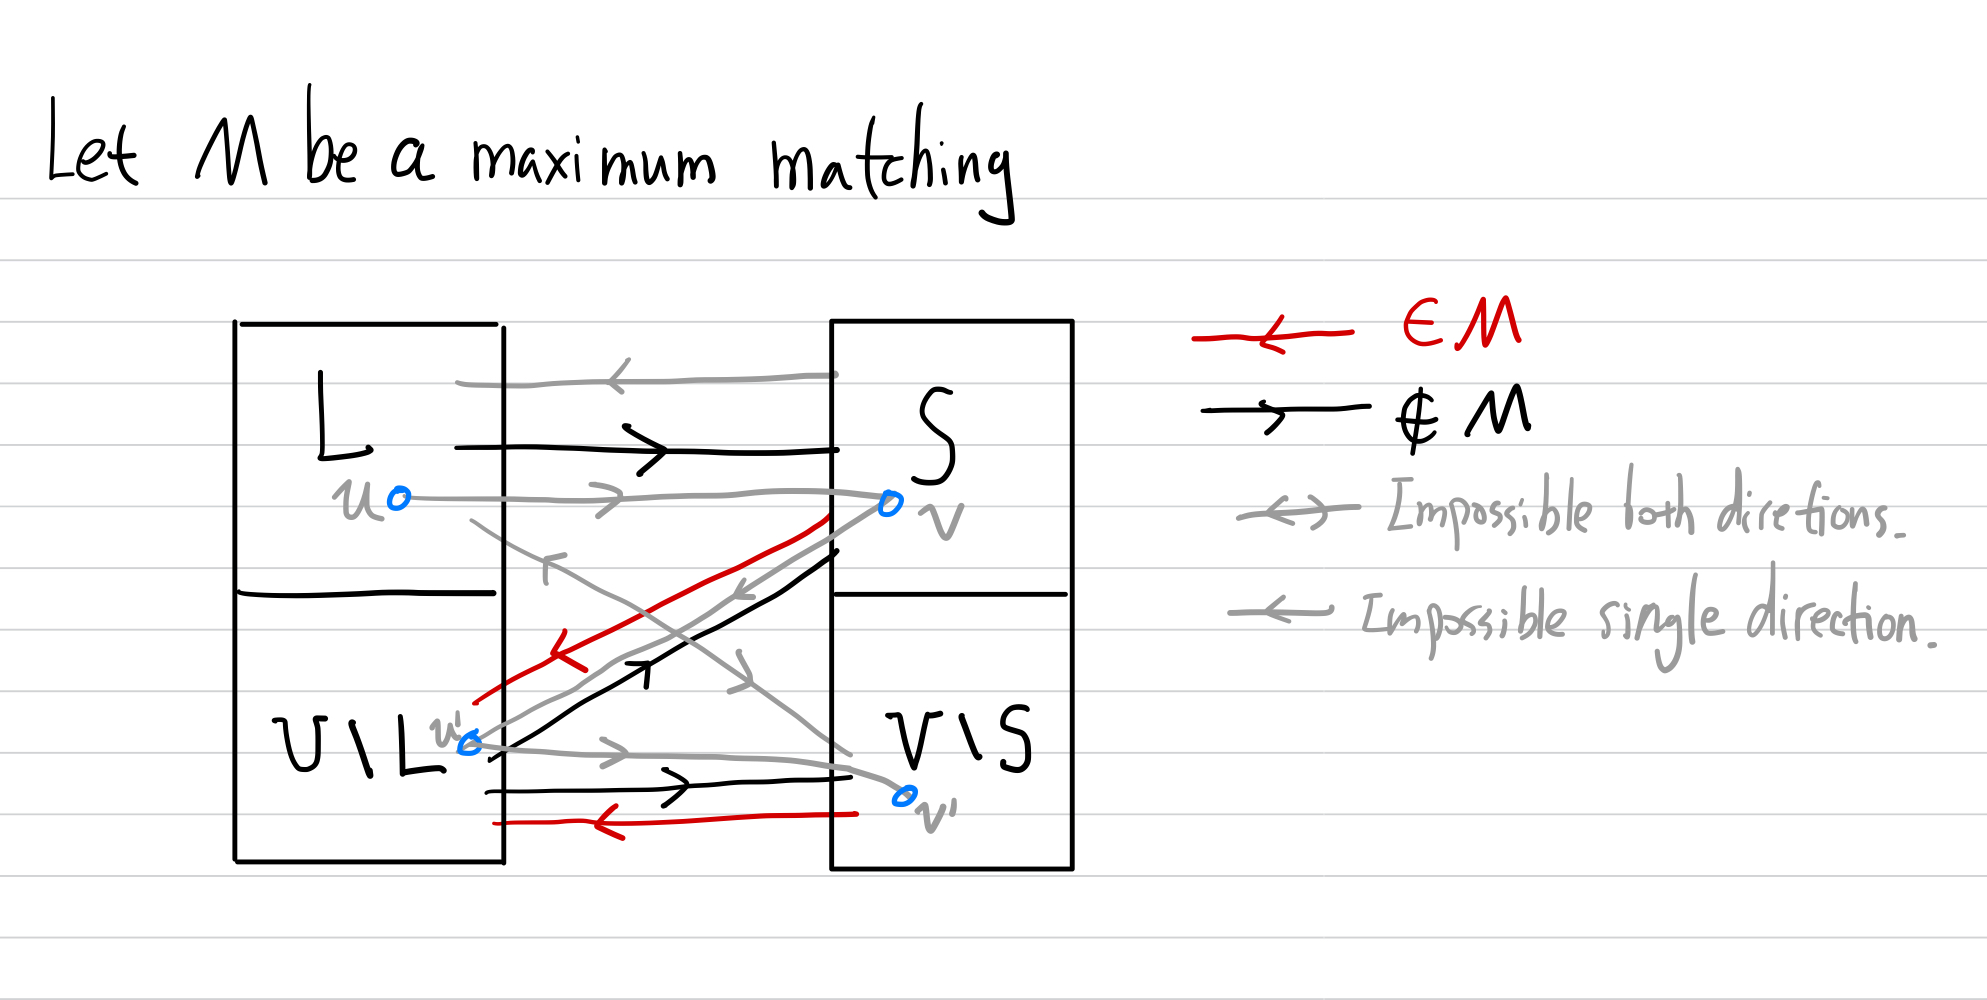
\includegraphics[width=12cm]{fig1.jpeg}
        \end{figure}
    \end{proof}

\section{Problem 3.25}


\section{Problem 8.4}
    Let $G = (V, E)$ be a graph. Describe the problem of finding a clique (= complete subgraph) of maximum cardinality as an integer linear programming problem. 
    \par
    We consider decision variables of both vertices and edges. Let $x\in [0, 1]^{|V|}$, then: 
    \begin{align}
        P & := \forall {u, v}\not \in E: 
                x_u + x_v \le 1
        \\
        P_I &:= P \cap \mathbb Z^{|E| + |V|} \leftarrow \text{This is what we want}
    \end{align}
    For every vertices chosen, there must exist an edge $e\in E$ between them, then it will be a clique on the graph. To assert it we prevent the case where $u, v$ are chosen and there is no edges betwee them (which is (2.0.1)). The second line (2.0.2) asserts the conditions that we want the integral solutions. 


\end{document}